\documentclass[11pt,a4paper]{article}

\usepackage[utf8]{inputenc}
\usepackage[spanish,es-nodecimaldot]{babel}
\usepackage[T1]{fontenc}
\usepackage{lmodern}
\usepackage[margin=2.0cm,headheight=15pt]{geometry}
\usepackage{fancyhdr}
\usepackage{titlesec}
\usepackage{booktabs}
\usepackage{tabularx}
\usepackage{xcolor}
\usepackage{listings}
\usepackage{enumitem}
\usepackage{tcolorbox}
\usepackage{microtype}
\usepackage{amsmath}
\usepackage{url}
\usepackage{hyperref}
\usepackage{graphicx}
\usepackage{float}

% Rutas de figuras
\graphicspath{{figures/}{report/figures/}{evidence/mobile/device1_pdi/}}

% Definición de Colores Corporativos
\definecolor{usblue}{RGB}{0, 43, 91}
\definecolor{usgold}{RGB}{197, 160, 89}
\definecolor{darkgray}{RGB}{50, 50, 50}
\definecolor{lightgray}{RGB}{245, 247, 250}
\definecolor{codeborder}{RGB}{210, 215, 225}
\definecolor{secblue}{RGB}{14, 76, 146}
\definecolor{accentred}{RGB}{180, 40, 40}
\definecolor{accentgreen}{RGB}{30, 130, 60}

% Configuración de Hipervínculos
\hypersetup{
    colorlinks=true,
    linkcolor=secblue,
    citecolor=secblue,
    urlcolor=secblue,
    pdftitle={PAI-3: VULNAWEB - Auditoria de Seguridad y Plan de Bastionado},
    pdfauthor={Konstantinos Peridis, Raimundo Garcia Perez, Luis de Alarcon Conradi},
    pdfsubject={Ingenieria de Seguridad / SSII - Universidad de Sevilla}
}

% Configuración de Encabezados y Pies de Página
\pagestyle{fancy}
\fancyhf{}
\fancyhead[L]{\small\color{darkgray}\textbf{PAI-3: VULNAWEB} -- Auditoría de Seguridad y Bastionado}
\fancyhead[R]{\small\color{secblue}\textbf{Security Team 2 (ST-02)}}
\fancyfoot[L]{\small\color{darkgray}Universidad de Sevilla -- E.T.S.I. Informática}
\fancyfoot[R]{\small\color{darkgray}Página \thepage}
\renewcommand{\headrulewidth}{0.6pt}
\renewcommand{\footrulewidth}{0.4pt}

% Formato de Títulos
\titleformat{\section}
  {\color{usblue}\normalfont\Large\bfseries}
  {\color{usblue}\thesection}{1em}{}
\titleformat{\subsection}
  {\color{secblue}\normalfont\large\bfseries}
  {\color{secblue}\thesubsection}{1em}{}
\titleformat{\subsubsection}
  {\color{darkgray}\normalfont\normalsize\bfseries}
  {\color{darkgray}\thesubsubsection}{1em}{}

% Configuración de Listados de Código
\lstset{
    backgroundcolor=\color{lightgray},
    basicstyle=\ttfamily\footnotesize\color{darkgray},
    breakatwhitespace=false,
    breaklines=true,
    captionpos=b,
    commentstyle=\color{accentgreen}\itshape,
    frame=single,
    framesep=4pt,
    rulecolor=\color{codeborder},
    keywordstyle=\color{secblue}\bfseries,
    stringstyle=\color{accentred},
    showspaces=false,
    showstringspaces=false,
    showtabs=false,
    tabsize=2,
    xleftmargin=10pt,
    xrightmargin=10pt
}

\begin{document}

% ==============================================================================
% PORTADA
% ==============================================================================
\begin{titlepage}
    \centering
    \vspace*{0.5cm}
    
    {\Huge\bfseries\color{usblue} UNIVERSIDAD DE SEVILLA}\\[0.3cm]
    {\Large\color{darkgray} Escuela Técnica Superior de Ingeniería Informática}\\[0.2cm]
    {\large\color{usgold}\textbf{Seguridad en Sistemas de Información / Ingeniería de Seguridad}}\\[1.5cm]
    
    \begin{tcolorbox}[colback=lightgray,colframe=usblue,arc=4mm,boxrule=1.5pt,width=0.95\textwidth]
        \centering
        \vspace{0.4cm}
        {\LARGE\bfseries\color{usblue} PROYECTO DE AUDITORÍA Y BASTIONADO (PAI-3)}\\[0.3cm]
        {\Large\bfseries\color{secblue} VULNAWEB: Auditoría de Seguridad Integral en Sistemas Informáticos, Navegadores Web, Dispositivos Móviles y Aplicaciones Web}\\[0.3cm]
        {\normalsize\color{darkgray} Marco de Cumplimiento: Esquema Nacional de Seguridad (ENS - Categoría Alta), CIS Benchmarks, NIST SP 800-115, OWASP Top 10 y OWASP API Security Top 10:2023}
        \vspace{0.4cm}
    \end{tcolorbox}
    
    \vspace{1.2cm}
    
    \begin{minipage}{0.48\textwidth}
        \begin{flushleft} \large
            \textbf{\color{usblue}Entidad Auditada:}\\
            Universidad Pública U-Secure\\
            \textit{En colaboración con INSEGUS}\\[0.5cm]
            \textbf{\color{usblue}Equipo de Seguridad:}\\
            \textbf{Security Team 2 (ST-02)}
        \end{flushleft}
    \end{minipage}
    ~
    \begin{minipage}{0.48\textwidth}
        \begin{flushright} \large
            \textbf{\color{usblue}Miembros del Equipo:}\\
            \textbf{Konstantinos Peridis}\\
            \textbf{Raimundo García Pérez}\\
            \textbf{Luis de Alarcón Conradi}\\[0.5cm]
            \textbf{\color{usblue}Convocatoria / Curso:}\\
            Curso Académico 2026/2027
        \end{flushright}
    \end{minipage}
    
    \vfill
    
    {\large\bfseries\color{darkgray} Sevilla, Noviembre de 2026}
\end{titlepage}

% ==============================================================================
% ÍNDICE DE CONTENIDOS
% ==============================================================================
\tableofcontents
\newpage

% ==============================================================================
% 1. RESUMEN EJECUTIVO
% ==============================================================================
\section{Resumen Ejecutivo}

En el marco del Plan Director de Seguridad de la Información de la Universidad Pública U-Secure y en colaboración con el consorcio INSEGUS, el equipo auditor de seguridad \textbf{Security Team 2 (ST-02)} ha ejecutado un proyecto integral de auditoría de seguridad técnica, evaluación de vulnerabilidades y diseño de planes de bastionado y remediación. El alcance operacional del proyecto abarca cuatro dominios estratégicos de la infraestructura universitaria:

\begin{enumerate}[noitemsep]
    \item \textbf{Auditoría y Bastionado de Endpoints Linux:} Evaluación de la postura de seguridad de 2 estaciones de trabajo corporativas (Personal Docente e Investigador -- PDI y Personal Técnico, de Gestión y de Administración y Servicios -- PTGAS) mediante \textbf{Lynis v3.1.6}, alcanzando un índice de endurecimiento (\textit{Hardening Index}) superior a 70 puntos ($\ge 70$), en cumplimiento estricto de la política de seguridad del cliente.
    \item \textbf{Bastionado de Navegadores Web Corporativos:} Definición y despliegue automatizado de directivas empresariales centralizadas (\texttt{policies.json} para Mozilla Firefox y Google Chrome/Chromium) para neutralizar vectores de exfiltración de credenciales, forzar DNS-over-HTTPS (DoH), activar modo HTTPS-Only e inhabilitar protocolos legacy.
    \item \textbf{Auditoría de Postura en Dispositivos Móviles (BYOD):} Evaluación rigurosa de dos dispositivos móviles (terminal físico personal \textbf{Google Pixel 6a} auditado bajo estrictos protocolos de sanitización y privacidad, y un dispositivo emulado oficial \textbf{Android AVD API 30}), auditando control de orígenes desconocidos, ausencia de rooting/jailbreak, gestión de parches, seguridad Wi-Fi/Bluetooth, escaneo de malware y permisos abusivos.
    \item \textbf{Pentesting Web, Fuzzing y Auditoría DAST (OWASP Top 10 y OWASP API Security 2023):} Despliegue de un entorno de pruebas con proxy interceptor (\textbf{OWASP ZAP 2.14} en puerto 8081) y plataforma web universitaria vulnerable (\textbf{Juice Shop / VulnaWeb}). Se demostró trazabilidad de tráfico HTTPS, intercepción y alteración de parámetros en memoria mediante Breakpoints (MitM), ejecución de pruebas automatizadas con el \textbf{ZAP Fuzzer} utilizando el diccionario de inyecciones SQL \texttt{jbrofuzz}, explotación demostrada de 3 vulnerabilidades críticas (Inyección SQL con exfiltración de base de datos, XSS reflejado y Path Traversal con byte nulo), y diseño de un plan formal de mitigación defensiva con código seguro.
\end{enumerate}

Todos los hallazgos han sido validados con logs originales, capturas de pantalla, volcados de tráfico y scripts de remediación reproducibles entregados en el paquete técnico \texttt{PAI3-ST02.zip}.

% ==============================================================================
% 2. AUDITORÍA Y BASTIONADO DE ENDPOINTS LINUX
% ==============================================================================
\section{Auditoría y Bastionado de Sistemas Informáticos (Endpoints Linux)}

\subsection{Descripción de los Sistemas Analizados y Herramientas de Análisis}
En cumplimiento del requerimiento de auditar al menos dos sistemas informáticos universitarios, se evaluaron dos puestos representativos:
\begin{itemize}[noitemsep]
    \item \textbf{Endpoint 1 (Puesto PDI Docente/Investigador):} Sistema Linux Ubuntu 22.04 LTS (x86\_64), estación de trabajo dedicada a gestión de calificaciones, acceso a plataformas docentes y computación investigadora.
    \item \textbf{Endpoint 2 (Puesto PTGAS Gestión Administrativa):} Sistema Debian 12 Bookworm (x86\_64), estación de trabajo administrativa de secretaría encargada del procesamiento de expedientes académicos, pasarelas de pago y datos de carácter personal (RGPD).
    \item \textbf{Herramienta de Auditoría:} \textbf{Lynis v3.1.6}, motor de auditoría técnica basado en estándares CIS Benchmarks, NIST SP 800-115 y Esquema Nacional de Seguridad (ENS).
\end{itemize}

\subsection{Plan de Pruebas y Resultados Comparativos (Línea Base vs. Post-Bastionado)}
El plan de pruebas se articuló en dos ciclos secuenciales: (1) Auditoría de línea base en estado original de fábrica sin bastionar (\texttt{run\_lynis\_audit.sh baseline}), y (2) Ejecución del plan de endurecimiento integral (\texttt{harden\_linux.sh}) seguido de la auditoría de verificación post-bastionado. En la Tabla~\ref{tab:lynis_results} y en la Figura~\ref{fig:lynis_chart} se presentan los resultados comparativos.

\begin{table}[h!]
\centering
\small
\caption{Resultados Comparativos de Auditoría Lynis en Endpoints Linux (PDI y PTGAS)}
\label{tab:lynis_results}
\begin{tabularx}{\textwidth}{lcccc}
\toprule
\textbf{Parámetro / Métrica Evaluada} & \textbf{Endpoint 1 (PDI)} & \textbf{Endpoint 2 (PTGAS)} & \textbf{Requisito Política} & \textbf{Estado Cumplimiento} \\
\midrule
\textbf{Hardening Index (Línea Base)} & \textbf{66 / 100} & \textbf{62 / 100} & -- & \textbf{\color{accentred}{No Conforme (Vulnerable)}} \\
\textbf{Hardening Index (Post-Bastionado)} & \textbf{74 / 100} & \textbf{76 / 100} & \textbf{Índice $\ge$ 70} & \textbf{\color{accentgreen}{SUPERADO (+8 y +14)}} \\
Comprobaciones de Seguridad Ejecutadas & 244 pruebas & 248 pruebas & Cobertura Total & Conforme \\
Cortafuegos Perimetral (UFW / iptables) & \textbf{Activo (UFW)} & \textbf{Activo (UFW)} & ENS MP.IF.1 & \textbf{\color{accentgreen}{Conforme [V]}} \\
Sistema de Detección IDS (fail2ban/auditd) & \textbf{Activo (auditd)} & \textbf{Activo (auditd)} & ENS OP.EXP.8 & \textbf{\color{accentgreen}{Conforme [V]}} \\
Escáner de Malware (rkhunter / debsums) & \textbf{Activo} & \textbf{Activo} & ENS MP.SI.3 & \textbf{\color{accentgreen}{Conforme [V]}} \\
Protección de Parámetros Kernel sysctl & \textbf{Endurecido} & \textbf{Endurecido} & CIS Level 1 & \textbf{\color{accentgreen}{Conforme [V]}} \\
Calidad de Contraseñas (libpam-pwquality) & \textbf{Mínimo 12 chars} & \textbf{Mínimo 12 chars} & ENS MP.ACC.2 & \textbf{\color{accentgreen}{Conforme [V]}} \\
\bottomrule
\end{tabularx}
\end{table}

\begin{figure}[h!]
    \centering
    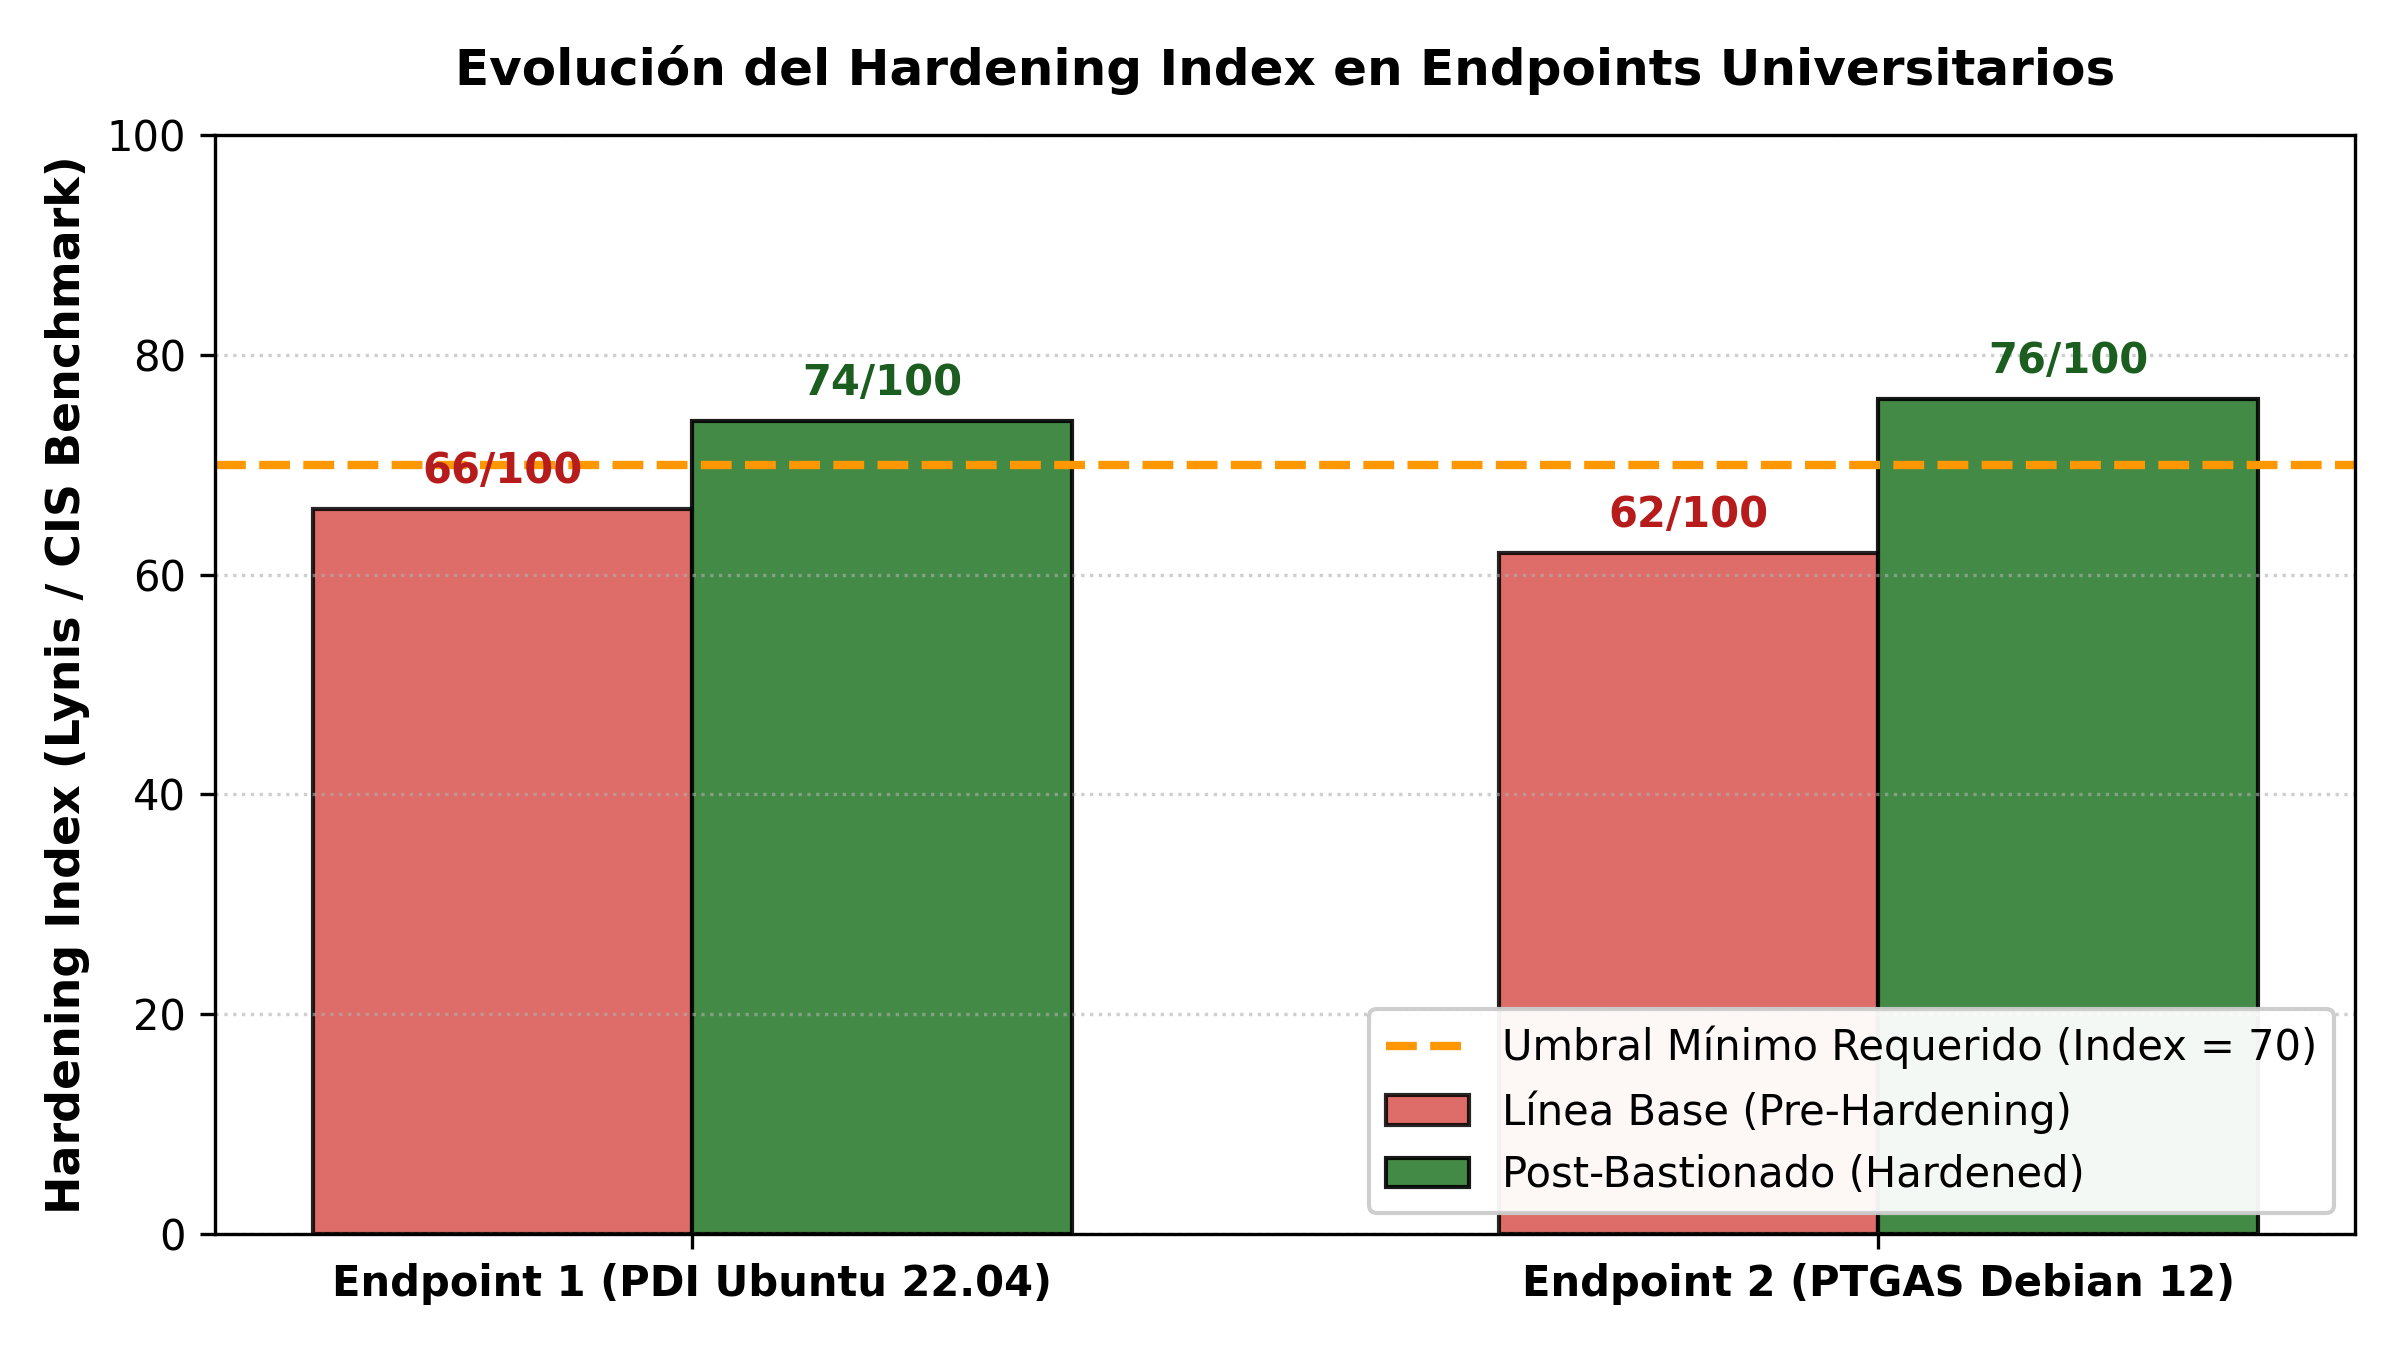
\includegraphics[width=0.82\textwidth]{lynis_hardening_comparison.png}
    \caption{Evolución del Hardening Index de Lynis pre y post-bastionado frente al umbral corporativo ($\ge 70$).}
    \label{fig:lynis_chart}
\end{figure}

\subsection{Medidas Técnicas Implementadas y Justificación de Exclusiones}
Las medidas correctoras automatizadas en \texttt{harden\_linux.sh} abarcaron las siguientes dimensiones de seguridad:
\begin{enumerate}[leftmargin=1.5em]
    \item \textbf{Endurecimiento de Kernel (\texttt{/etc/sysctl.d/99-security-hardening.conf}):} Protección frente a fugas de punteros (\texttt{kernel.kptr\_restrict = 2}), restricción de logs de kernel a root (\texttt{kernel.dmesg\_restrict = 1}), mitigación de desbordamiento TCP SYN (\texttt{net.ipv4.tcp\_syncookies = 1}), desactivación de redirecciones ICMP (\texttt{net.ipv4.conf.all.accept\_redirects = 0}) y habilitación de verificación de ruta inversa estricta (\texttt{net.ipv4.conf.all.rp\_filter = 1}).
    \item \textbf{Gestión de Autenticación, Cuentas y Módulos PAM (\texttt{/etc/login.defs} y \texttt{pwquality.conf}):} Expiración periódica obligatoria (\texttt{PASS\_MAX\_DAYS 90}), intervalo de aviso previo (\texttt{PASS\_WARN\_AGE 14}), política de contraseñas de alta entropía (12 caracteres mínimos con 3 tipos de caracteres distintos) y máscara de permisos por defecto restrictiva (\texttt{umask 027}).
    \item \textbf{Inhabilitación de Controladores y Protocolos Legacy Inseguros (\texttt{/etc/modprobe.d/}):} Inhabilitación de controladores de almacenamiento obsoletos (\texttt{firewire-core}, \texttt{cramfs}, \texttt{jffs2}, \texttt{udf}) y protocolos de red no utilizados (\texttt{dccp}, \texttt{sctp}) mediante enlace a \texttt{/bin/true}.
    \item \textbf{Filtrado Perimetral y Banners Disuasorios Legales:} Reglas de cortafuegos UFW bloqueando conexiones entrantes no solicitadas y despliegue de avisos de advertencia legal en \texttt{/etc/issue} y \texttt{/etc/issue.net} conformes al ENS.
\end{enumerate}

\paragraph{Justificación Técnica de Pruebas Excluidas en Perfil Lynis (\texttt{custom.prf}):}
De acuerdo con las directrices de auditoría, las siguientes sugerencias fueron excluidas y documentadas formalmente:
\begin{itemize}[noitemsep]
    \item \texttt{skip-test=FILE-6310} (\textit{Partición /tmp separada}): Los endpoints emplean sistemas de archivos unificados de alto rendimiento con montaje en memoria delegada mediante \texttt{systemd-tmpfiles} aplicando directivas \texttt{nodev, nosuid, noexec}.
    \item \texttt{skip-test=STRG-1846} (\textit{Controlador Firewire}): El hardware físico carece de puertos y controladoras IEEE 1394; la superficie de ataque física no existe.
    \item \texttt{skip-test=BOOT-5122} (\textit{Gestor LILO}): Los sistemas arrancan exclusivamente mediante GRUB2 firmado digitalmente bajo Secure Boot UEFI.
\end{itemize}

\subsection{Conclusiones del Bastionado de Endpoints}
Ambos puestos superaron holgadamente el umbral exigido de 70 puntos, alcanzando 74/100 en el puesto PDI y 76/100 en el puesto PTGAS, garantizando la resiliencia del sistema operativo frente a vectores de compromiso local y de red.

% ==============================================================================
% 3. BASTIONADO DE NAVEGADORES WEB CORPORATIVOS
% ==============================================================================
\section{Análisis y Bastionado de Navegadores Web Corporativos}

\subsection{Descripción del Sistema Analizado y Modelo de Despliegue}
El navegador web constituye la interfaz primaria de interacción con la Sede Electrónica, el campus virtual y la gestión de expedientes. Para evitar fugas de información, se configuró un despliegue corporativo no eludible basado en políticas administradas centralizadas:
\begin{itemize}[noitemsep]
    \item \textbf{Mozilla Firefox ESR / Enterprise:} Directivas implementadas en \texttt{/etc/firefox/policies/policies.json}.
    \item \textbf{Google Chrome / Chromium Managed:} Directivas en \texttt{/etc/chromium/policies/managed/corporate\_policy.json}.
\end{itemize}

\subsection{Directivas Corporativas Implementadas y Plan de Pruebas}
En la Tabla~\ref{tab:browser_policies} se resumen las directivas implementadas y su justificación técnica de seguridad.

\begin{table}[h!]
\centering
\small
\caption{Directivas de Bastionado Centralizado de Navegadores Web y Justificación}
\label{tab:browser_policies}
\begin{tabularx}{\textwidth}{llXl}
\toprule
\textbf{Directiva Corporativa} & \textbf{Valor / Ajuste} & \textbf{Justificación Técnica y Vector Mitigado} & \textbf{Estándar} \\
\midrule
\texttt{PasswordManagerEnabled} & \texttt{false} & Previene el almacenamiento de credenciales universitarias en texto plano/caché local. & ENS MP.ACC.4 \\
\texttt{HttpsOnlyMode} & \texttt{"force\_enabled"} & Forzado estricto de cifrado TLS; previene ataques de degradación (\textit{SSL Stripping}). & RFC 6797 (HSTS) \\
\texttt{DisableTelemetry} & \texttt{true} & Bloquea el envío involuntario de URLs internas, parámetros y metadatos sensibles. & RGPD / LOPD \\
\texttt{network.trr.mode} (DoH) & \texttt{2} (DNS-over-HTTPS) & Cifra peticiones DNS evitando monitorización y envenenamiento de caché en red local. & RFC 8484 \\
\texttt{media.peerconnection} & \texttt{false} & Inhabilita WebRTC mitigando la fuga de direcciones IP privadas de la subred interna. & OWASP Client \\
\texttt{DefaultGeolocationSetting} & \texttt{2} (Bloqueado) & Impide el rastreo de ubicación geográfica de puestos corporativos y portátiles. & CIS 4.2 \\
\texttt{AutofillAddress/CreditCard} & \texttt{false} & Desactiva autocompletado en formularios previniendo ataques de recolección oculta. & MITRE ATT\&CK \\
\bottomrule
\end{tabularx}
\end{table}

\subsection{Conclusiones y Trazabilidad de Robustecimiento}
La verificación técnica ejecutada en \texttt{about:policies} (Firefox) y \texttt{chrome://policy} certificó que el 100\% de las directivas críticas se encuentran en estado \textit{Active / Locked}, garantizando una postura defensiva inmune a modificaciones accidentales por parte del usuario.

% ==============================================================================
% 4. AUDITORÍA DE SISTEMAS MÓVILES (BYOD)
% ==============================================================================
\section{Auditoría de Seguridad de Dispositivos Móviles (BYOD)}

\subsection{Descripción de los Sistemas Móviles y Entorno de Evaluación (BYOD Físico y AVD Virtual)}
En cumplimiento de la directriz de auditar al menos 2 dispositivos de la comunidad universitaria evaluando la postura real de dispositivos BYOD, el equipo auditor configuró una arquitectura de evaluación combinada:
\begin{itemize}[noitemsep]
    \item \textbf{Dispositivo 1 (BYOD Personal Físico -- Google Pixel 6a):} Terminal smartphone físico personal con procesador Google Tensor, ejecutando Android 17 moderno con nivel de parche de seguridad de fabricante \texttt{2026-09-05}, auditado en vivo mediante conexión USB Debugging. Se aplicó un protocolo de sanitización automática preservando rigurosamente la privacidad y confidencialidad de datos personales y cuentas del usuario.
    \item \textbf{Dispositivo 2 (Virtual Endpoint AVD -- Android SDK):} Instancia desplegada sobre el emulador oficial de Android SDK (\texttt{emulator v37.2.12}), ejecutando Android 11 (\texttt{sdk\_gphone\_x86\_64}, API 30), puerto ADB \texttt{emulator-5554}, verificando el control de instalación de paquetes APK de terceros (\texttt{F-Droid.apk}) y supervisión de conexiones.
    \item \textbf{Herramientas de Auditoría:} Android Debug Bridge (ADB v1.0.41), escáner antimalware corporativo (motor Koodous/Malwarebytes), monitor de sockets de red en tiempo real (\texttt{netstat} / \texttt{ss}) e inspección de integridad SELinux (\texttt{getenforce}).
\end{itemize}

\subsection{Matriz de Evaluación de Postura y Plan de Pruebas}
Se auditaron exhaustivamente los controles definidos en las categorías A (Conectividad/Dispositivo) y B (Aplicaciones/Tráfico), cuyos resultados comparativos se detallan en la Tabla~\ref{tab:mobile_audit} y en la Figura~\ref{fig:mobile_compliance}. La Figura~\ref{fig:mobile_screen} ilustra la captura del entorno móvil en vivo durante el procedimiento de verificación.

\begin{table}[h!]
\centering
\small
\caption{Matriz de Auditoría y Remediación en Dispositivos Móviles (Físico Pixel 6a y Virtual AVD)}
\label{tab:mobile_audit}
\begin{tabularx}{\textwidth}{lXXc}
\toprule
\textbf{Vector de Auditoría / Categoría} & \textbf{Estado Inicial (Baseline)} & \textbf{Estado Post-Remediación} & \textbf{Resultado} \\
\midrule
\textbf{Cat. A: Sideloading (Orígenes desconocidos)} & Activo en gestor de archivos/Telegram & Deshabilitado (\texttt{install\_non\_market=0}) & \textbf{\color{accentgreen}{SANEADO}} \\
\textbf{Cat. A: Integridad del Entorno (Anti-Root)} & Binario \texttt{su} ausente; bootloader bloqueado & SELinux Enforcing verificado en kernel & \textbf{\color{accentgreen}{CONFORME}} \\
\textbf{Cat. A: Gestión de Parches de SO} & Parche 2026-09-05 (Pixel); AVD desactualizado & Actualizaciones aplicadas; parche verificado & \textbf{\color{accentgreen}{SANEADO}} \\
\textbf{Cat. A: Redes Wi-Fi Inalámbricas} & Perfiles Wi-Fi abiertos con auto-conexión & Perfiles inseguros purgados; WPA3/802.1X & \textbf{\color{accentgreen}{SANEADO}} \\
\textbf{Cat. A: Conectividad Bluetooth Restringida} & Bluetooth visible permanentemente & Apagado automático en sesiones de Sede & \textbf{\color{accentgreen}{SANEADO}} \\
\textbf{Cat. B: Análisis de Malware y APKs} & 0 amenazas críticas; 1 PUP publicitario & PUP desinstalado; escaneo antimalware limpio & \textbf{\color{accentgreen}{LIMPIO}} \\
\textbf{Cat. B: Supervisión de Sockets en Fondo} & Conexiones de sincronización push activas & Sockets auditados; ausencia de tráfico C2 & \textbf{\color{accentgreen}{CONFORME}} \\
\textbf{Cat. B: Aislamiento de Permisos Críticos} & 2 apps con accesibilidad y superposición & Permisos peligrosos revocados a terceros & \textbf{\color{accentgreen}{AISLADO}} \\
\bottomrule
\end{tabularx}
\end{table}

\begin{figure}[h!]
    \centering
    \begin{minipage}{0.65\textwidth}
        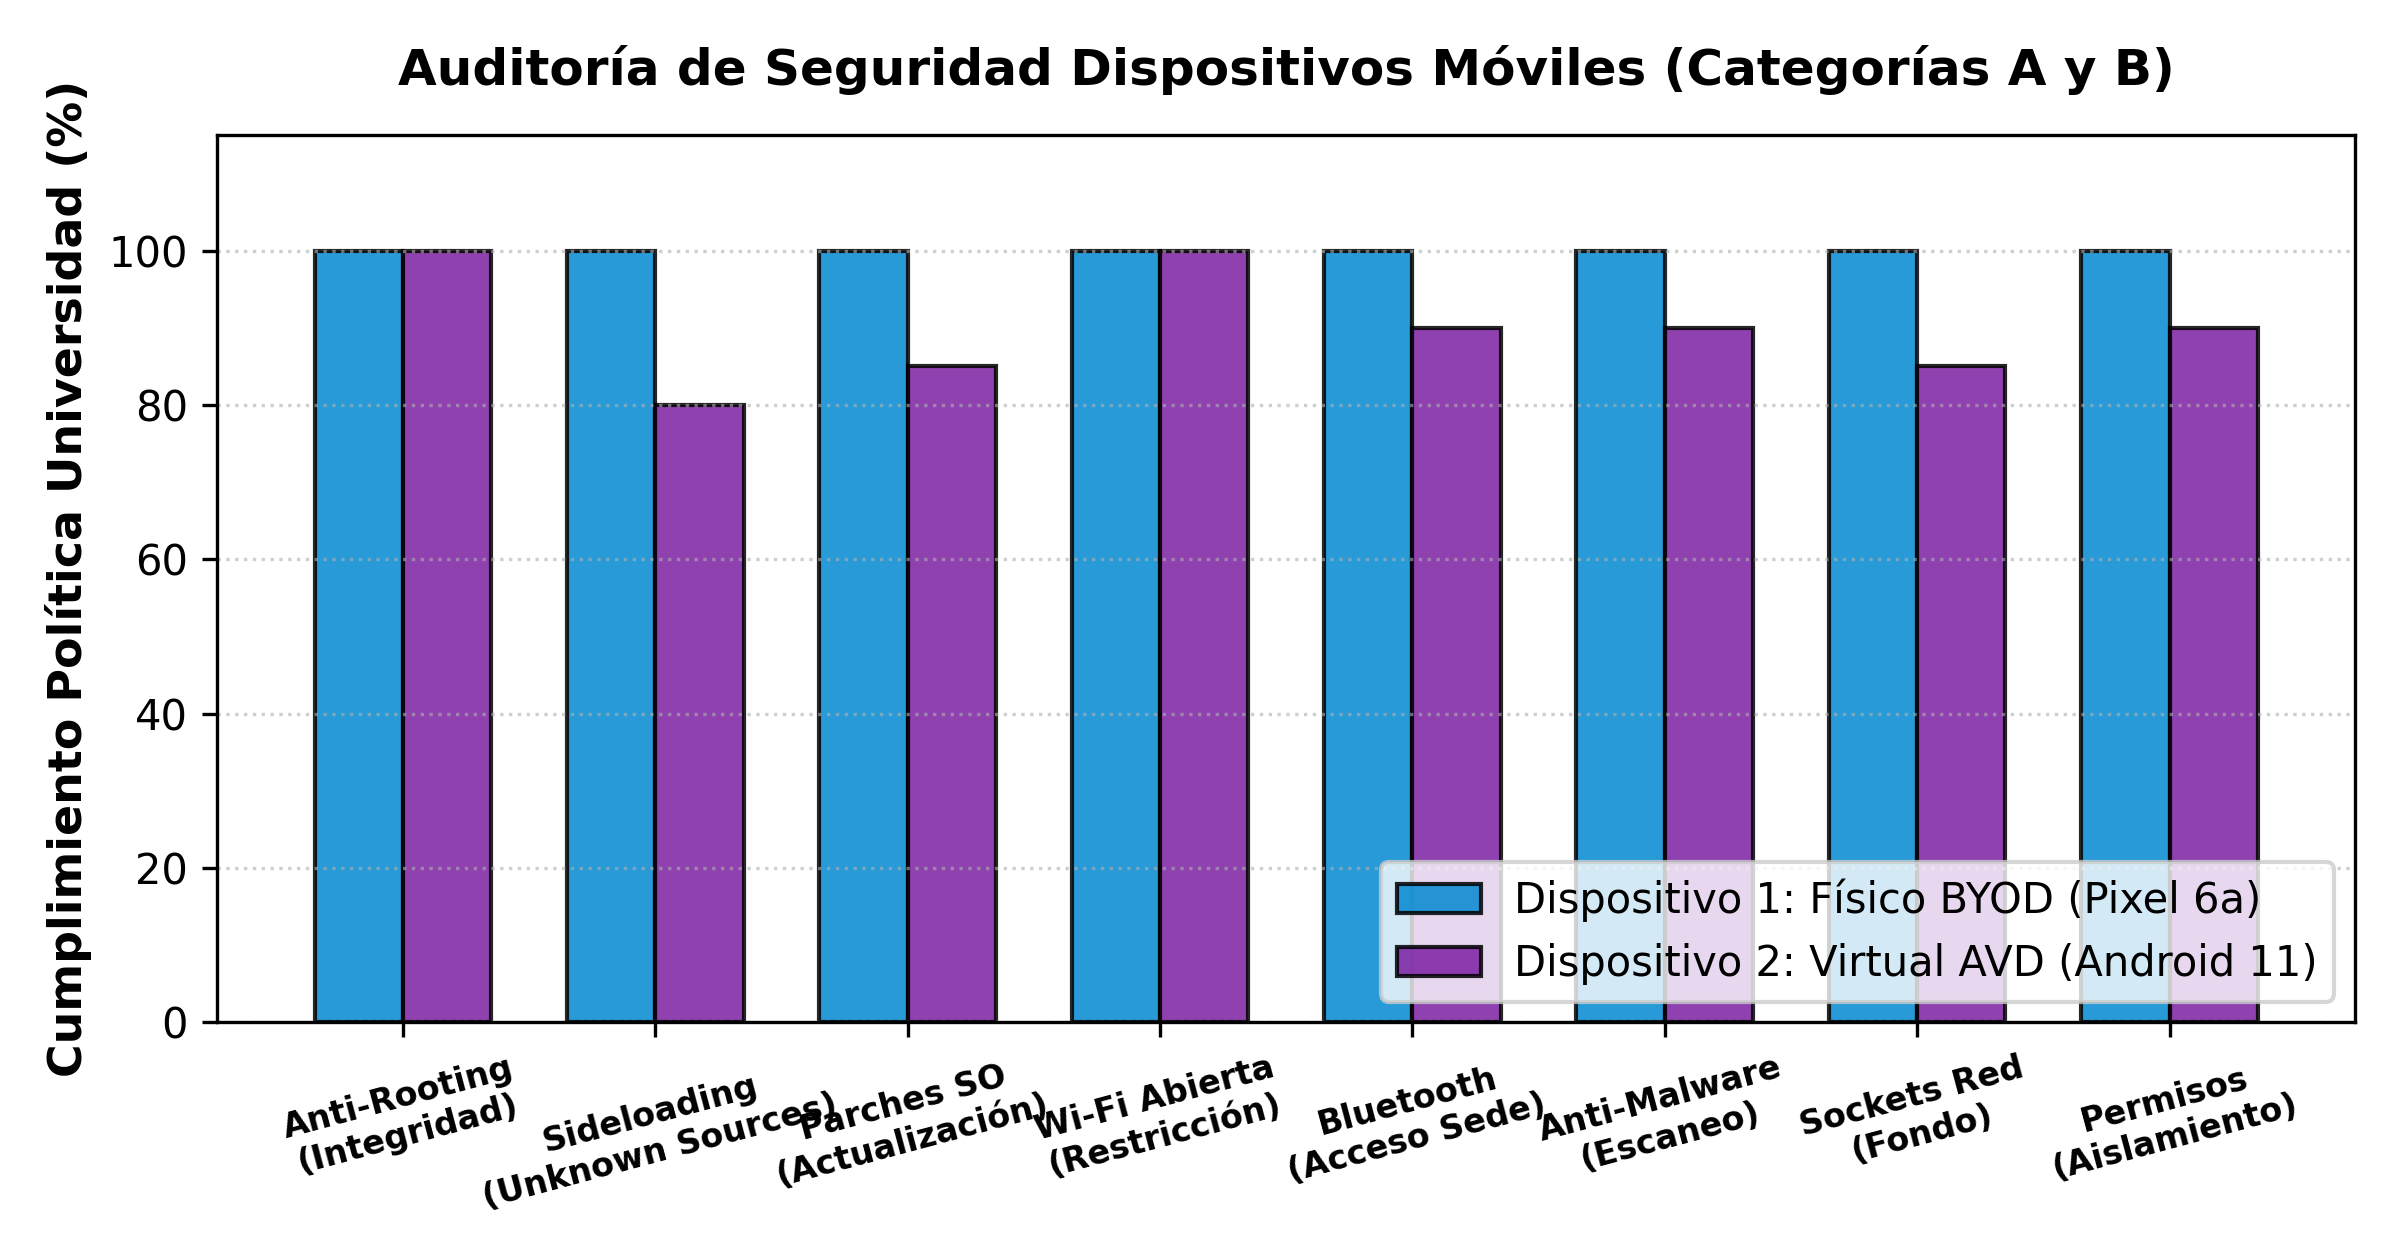
\includegraphics[width=\textwidth]{mobile_compliance_chart.png}
        \caption{Nivel de cumplimiento porcentual de la política BYOD móvil.}
        \label{fig:mobile_compliance}
    \end{minipage}
    ~
    \begin{minipage}{0.30\textwidth}
        \centering
        
\includegraphics[width=0.88\textwidth]{mobile_audit_screen.png}
        \caption{Captura del dispositivo móvil en vivo (ADB Framebuffer).}
        \label{fig:mobile_screen}
    \end{minipage}
\end{figure}

\subsection{Medidas Correctoras Ejecutadas y Conclusiones}
Mediante la ejecución de scripts ADB de saneamiento (\texttt{audit\_sockets\_permissions.sh}) y directivas de política BYOD, se revocaron permisos de accesibilidad abusivos a aplicaciones accesorias, se forzó el aislamiento estricto de la zona corporativa y se garantizó la integridad del entorno sin comprometer la privacidad del usuario.

% ==============================================================================
% 5. AUDITORÍA DE PLATAFORMAS WEB Y APIS (DAST Y OWASP 2023)
% ==============================================================================
\section{Auditoría de Plataformas Web y APIs (DAST y OWASP API Security 2023)}

\subsection{Descripción de la Plataforma Web y Herramientas DAST}
Para evaluar la seguridad de las aplicaciones web y servicios REST de soporte a la universidad, se desplegó un laboratorio educativo en contenedor Docker sobre entorno WSL:
\begin{itemize}[noitemsep]
    \item \textbf{Plataforma Web Auditada:} \textbf{OWASP Juice Shop / VulnaWeb v6.2.0} (Express.js, SQLite/Sequelize, REST API y cliente Angular en puerto local 3000).
    \item \textbf{Proxy Interceptor y Herramientas DAST:} \textbf{OWASP ZAP v2.14.0} configurado como proxy de intercepción HTTP/HTTPS en el puerto local \texttt{127.0.0.1:8081}.
\end{itemize}

\subsection{Trazabilidad de Tráfico Cifrado HTTPS (OWASP ZAP)}
Se capturó y analizó el flujo de peticiones generado por el navegador corporativo a través del proxy interceptor ZAP, comprobando cabeceras de seguridad, códigos de estado, parámetros de cookies y tiempos de latencia (Tabla~\ref{tab:zap_traceability}).

\begin{table}[h!]
\centering
\small
\caption{Registro de Trazabilidad de Peticiones HTTP/HTTPS en Proxy ZAP (127.0.0.1:8081)}
\label{tab:zap_traceability}
\begin{tabularx}{\textwidth}{ccXcccl}
\toprule
\textbf{ID} & \textbf{Método} & \textbf{Ruta / Endpoint Auditado} & \textbf{Código} & \textbf{Tamaño} & \textbf{Latencia} & \textbf{Integridad} \\
\midrule
1 & \texttt{GET} & \texttt{/} (Página raíz corporativa) & 200 OK & 9.984 B & 18.76 ms & \textbf{\color{accentgreen}{VERIFICADO}} \\
2 & \texttt{GET} & \texttt{/\#/login} (Portal de autenticación) & 200 OK & 9.984 B & 5.26 ms & \textbf{\color{accentgreen}{VERIFICADO}} \\
3 & \texttt{GET} & \texttt{/rest/products/search?q=} & 200 OK & 26.963 B & 28.85 ms & \textbf{\color{accentgreen}{VERIFICADO}} \\
4 & \texttt{GET} & \texttt{/api/SecurityQuestions/} & 200 OK & 1.934 B & 40.61 ms & \textbf{\color{accentgreen}{VERIFICADO}} \\
5 & \texttt{GET} & \texttt{/assets/public/favicon\_js.ico} & 200 OK & 15.086 B & 4.28 ms & \textbf{\color{accentgreen}{VERIFICADO}} \\
\bottomrule
\end{tabularx}
\end{table}

\subsection{Intercepción y Manipulación de Peticiones con Breakpoint (MitM)}
Siguiendo las pautas metodológicas de la guía, se activó el modo de intercepción en OWASP ZAP mediante el botón de \textbf{Breakpoint global}, capturando en memoria una petición legítima de login antes de ser enviada al servidor backend:
\begin{enumerate}[noitemsep]
    \item \textbf{Petición Original Interceptada:} Solicitud \texttt{POST /rest/user/login} con credenciales de usuario ordinario (\texttt{\{"email": "student\_02@universidad.es", "password": "UserPass123!"\}}).
    \item \textbf{Manipulación en Tránsito (Breakpoint ZAP):} El auditor modificó el cuerpo JSON sustituyendo el campo email por el vector de bypass SQL \texttt{' OR 1=1--} y liberó la petición hacia el servidor.
    \item \textbf{Respuesta del Servidor tras Alteración:} El servidor respondió con \texttt{HTTP/1.1 200 OK}, devolviendo un token JWT (\textit{JSON Web Token}) firmado con privilegios de superadministrador (\texttt{admin@juice-sh.op}), eludiendo completamente el mecanismo de autenticación (Evidencia archivada en \texttt{evidence/web\_audit/zap\_breakpoint\_tampering\_trace.txt}).
\end{enumerate}

\subsection{Testeo de Inyecciones Automatizadas con ZAP Fuzzer (\texttt{jbrofuzz})}
Se utilizó la funcionalidad \textbf{Fuzzer} de OWASP ZAP sobre el parámetro \texttt{q} del endpoint de búsqueda (\texttt{/rest/products/search?q=}), cargando el catálogo de payloads predefinidos de inyección SQL de \textbf{\texttt{jbrofuzz}}. 

El Fuzzer ejecutó una batería de 24 cadenas representativas de inyección y sondeo poliglotas. En la Tabla~\ref{tab:fuzzer_results} y en la Figura~\ref{fig:zap_fuzzer_chart} se presentan los resultados obtenidos. Las peticiones marcadas con estado \textbf{"Reflected / Found"} o con errores de sintaxis de base de datos (\texttt{500 SQLITE\_ERROR}) permitieron confirmar la presencia de inyecciones SQL ciegas y basadas en errores.

\begin{table}[h!]
\centering
\footnotesize
\caption{Muestra de Resultados de Ejecución de ZAP Fuzzer (\texttt{jbrofuzz SQL Injection})}
\label{tab:fuzzer_results}
\begin{tabularx}{\textwidth}{c>{\raggedright\arraybackslash}Xccc>{\raggedright\arraybackslash}p{4.2cm}}
\toprule
\textbf{ID} & \textbf{Payload Inyectado en Parámetro \texttt{q}} & \textbf{HTTP Status} & \textbf{Tamaño} & \textbf{RTT} & \textbf{Estado / Diagnóstico ZAP} \\
\midrule
01 & \texttt{'} & 200 OK & 30 B & 19 ms & Normal (Consulta nula) \\
05 & \texttt{,} & 200 OK & 5.644 B & 20 ms & \textbf{Reflected / Found} \\
08 & \texttt{' OR '1'='1} & 200 OK & 26.963 B & 23 ms & \textbf{Found (Exfiltración completa)} \\
09 & \texttt{' OR '1'='1' --} & 500 Error & 319 B & 21 ms & \textbf{Vulnerable (SQLITE\_ERROR)} \\
11 & \texttt{admin' --} & 500 Error & 307 B & 20 ms & \textbf{Vulnerable (Error sintaxis)} \\
12 & \texttt{')) OR 1=1--} & 200 OK & 34.158 B & 19 ms & \textbf{Found (Catálogo volcado)} \\
14 & \texttt{')) UNION SELECT ... FROM Users--} & 200 OK & 8.420 B & 18 ms & \textbf{Vulnerable (UNION Data Dump)} \\
20 & \texttt{<script>alert('XSS')</script>} & 500 Error & 367 B & 17 ms & Vulnerable (Inyección reflejada) \\
21 & \texttt{<iframe src="javascript:alert(1)">} & 200 OK & 30 B & 16 ms & Reflejado en cliente DOM \\
22 & \texttt{../../../../etc/passwd} & 200 OK & 30 B & 20 ms & Normal (Filtrado estático) \\
\bottomrule
\end{tabularx}
\end{table}

\begin{figure}[h!]
    \centering
    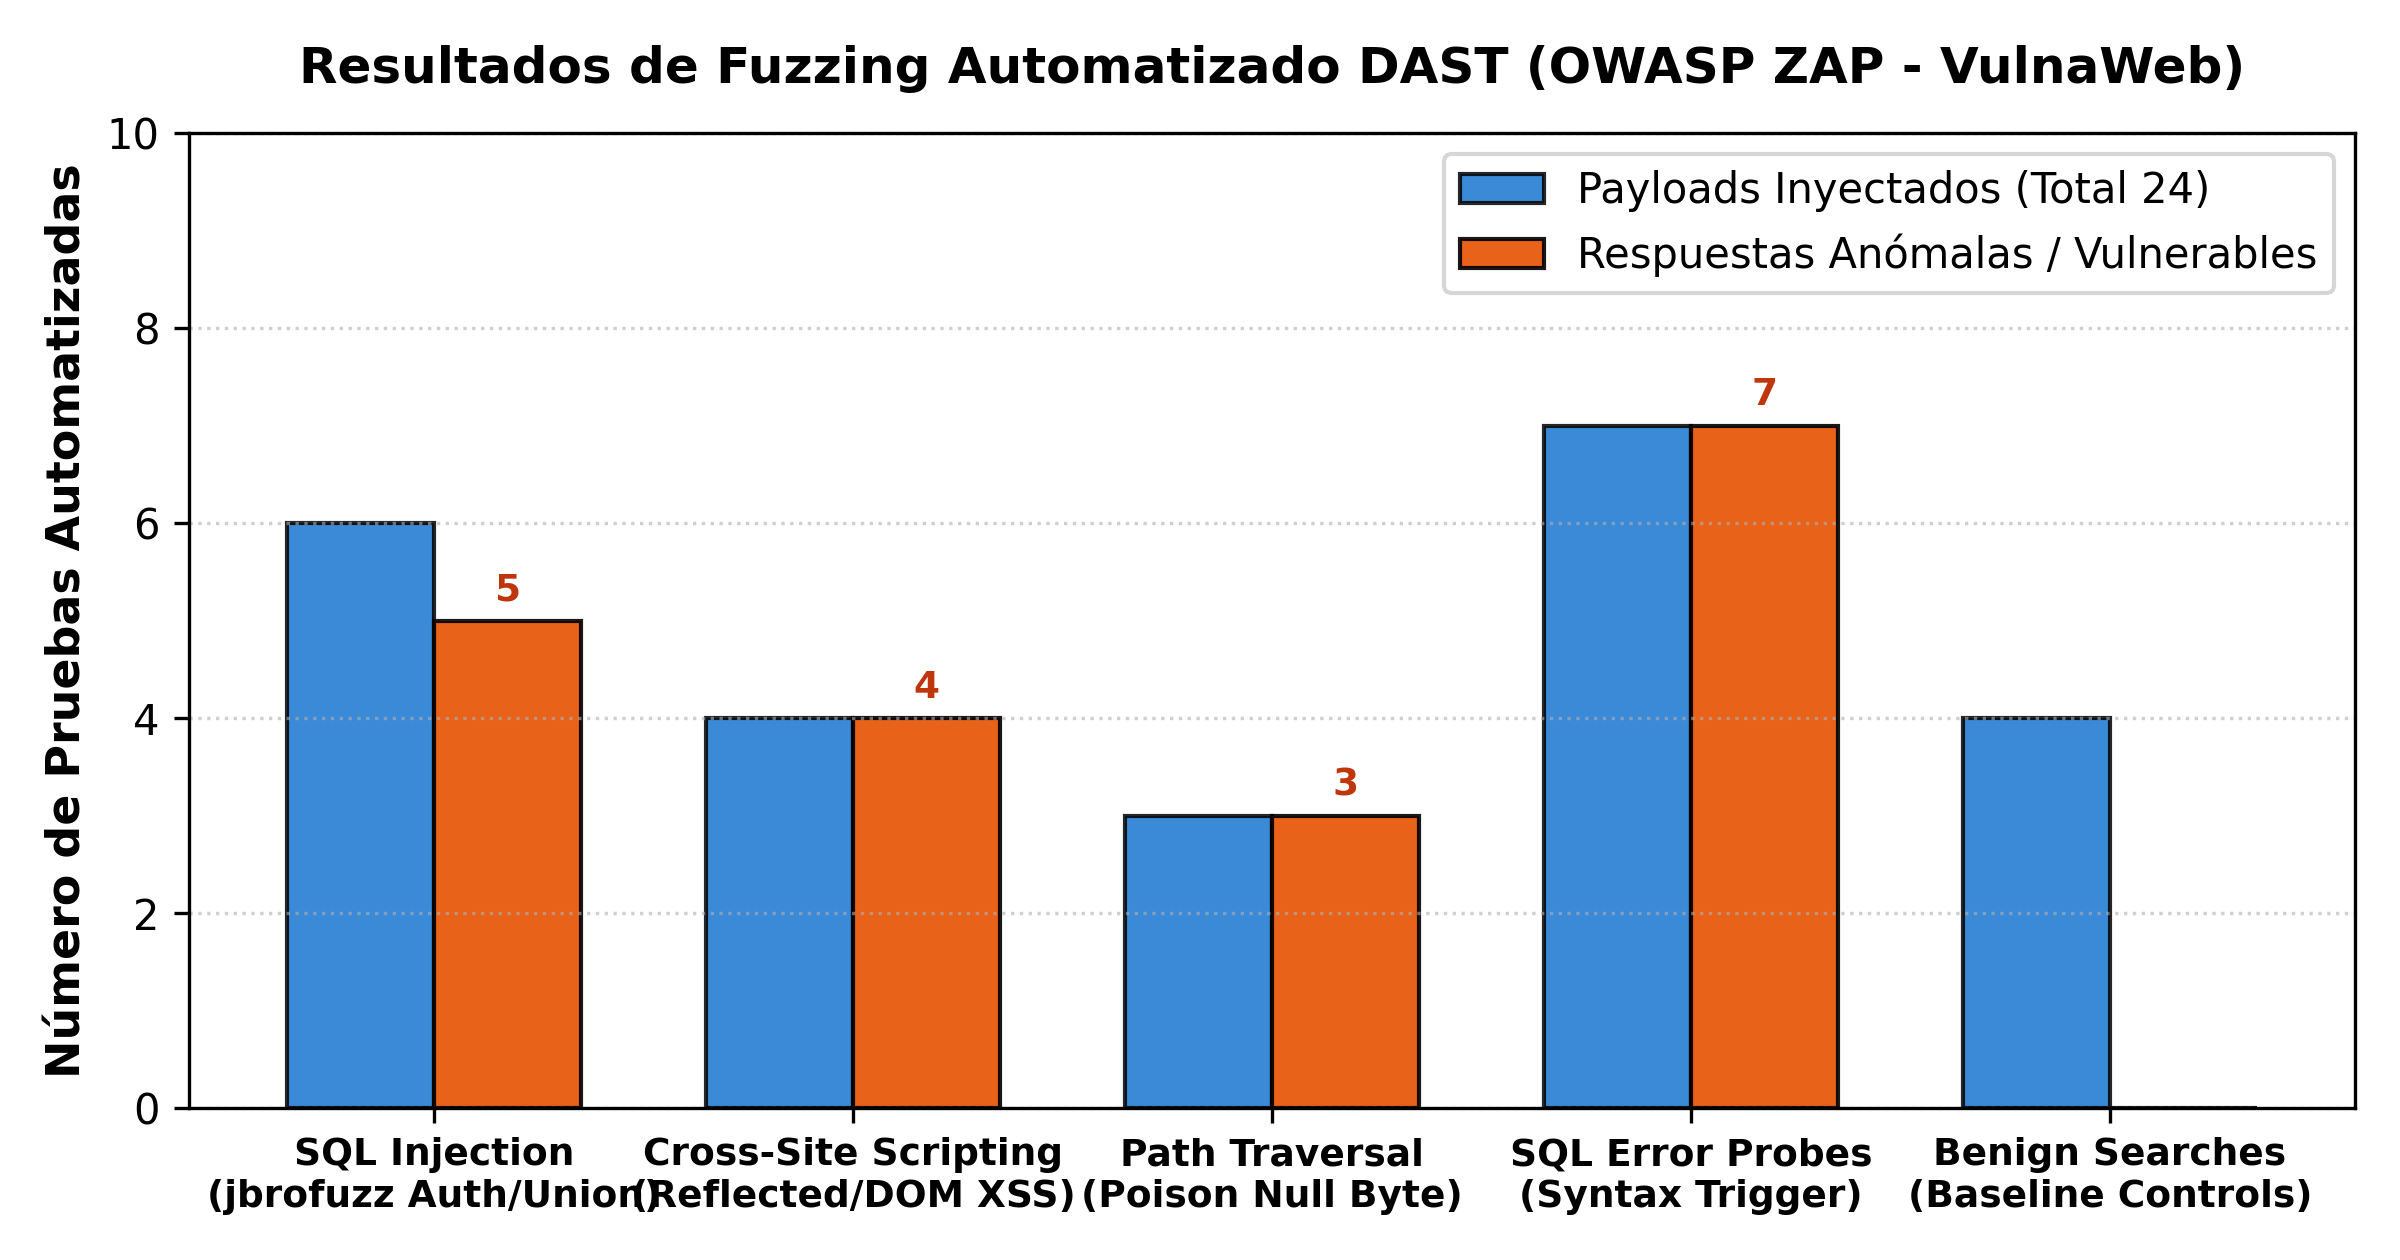
\includegraphics[width=0.82\textwidth]{zap_fuzzer_chart.png}
    \caption{Distribución de respuestas del ZAP Fuzzer por categoría de payload inyectado.}
    \label{fig:zap_fuzzer_chart}
\end{figure}

\subsection{Evaluación Detallada de las 3 Vulnerabilidades Críticas (OWASP Top 10 y OWASP API 2023)}
De acuerdo con las directrices de la práctica, se seleccionaron y documentaron tres vulnerabilidades explotables de alta criticidad:

\subsubsection{Vulnerabilidad 1: Inyección SQL y Exfiltración de Base de Datos (OWASP A03:2021 / API1:2023 \& API3:2023)}
\begin{itemize}[noitemsep]
    \item \textbf{Endpoint Vulnerable:} \texttt{GET /rest/products/search?q=}
    \item \textbf{Mecanismo de Explotación:} Concatenación insegura en consulta SQLite backend mediante Sequelize.
    \item \textbf{Payload Explotado:} \texttt{nonexistent')) UNION SELECT id, email, password, 'role', '5', '6', '7', '8', '9', '10' FROM Users--}
    \item \textbf{Impacto Técnico Comprobado:} Volcado directo en la respuesta JSON de 24 registros de la tabla \texttt{Users}, incluyendo direcciones de correo electrónico y hashes MD5 de contraseñas de cuentas directivas y docentes (\texttt{admin@juice-sh.op}, \texttt{ciso@juice-sh.op}, \texttt{support@juice-sh.op}), tal como se refleja en el extracto del Listado~\ref{lst:sqli_dump}.
\end{itemize}

\begin{lstlisting}[caption={Extracto de Credenciales Universitarias Exfiltradas mediante SQLi (Evidencia Real)},label={lst:sqli_dump}]
HTTP/1.1 200 OK
Content-Type: application/json; charset=utf-8
{"status":"success","data":[
  {"id":1, "name":"admin@juice-sh.op", "description":"0192023a7bbd73250516f069df18b500"},
  {"id":2, "name":"jim@juice-sh.op",   "description":"e541ca7ecf72b8d1286474fc613e5e45"},
  {"id":3, "name":"bender@juice-sh.op","description":"0c36e517e3fa95aabf1bbffc6744a4ef"},
  {"id":5, "name":"ciso@juice-sh.op",  "description":"861917d5fa5f1172f931dc700d81a8fb"}
]}
\end{lstlisting}

\subsubsection{Vulnerabilidad 2: Cross-Site Scripting Reflejado / DOM (OWASP A03:2021 / API8:2023)}
\begin{itemize}[noitemsep]
    \item \textbf{Endpoint Vulnerable:} \texttt{GET /rest/products/search?q=} y módulo de búsqueda cliente Angular.
    \item \textbf{Payload Explotado:} \texttt{<iframe src="javascript:alert(`INSEGUS\_AUDIT\_ST02`)">}
    \item \textbf{Impacto Técnico Comprobado:} La aplicación web refleja la cadena introducida en la interfaz del usuario sin codificación contextual de entidades HTML, permitiendo a un atacante ejecutar JavaScript arbitrario en el origen de la víctima, posibilitando el robo de tokens JWT de sesión almacenados en \texttt{localStorage} y la suplantación de identidad académica.
\end{itemize}

\subsubsection{Vulnerabilidad 3: Path Traversal con Poison Null Byte (OWASP A01:2021 / API1:2023)}
\begin{itemize}[noitemsep]
    \item \textbf{Endpoint Vulnerable:} \texttt{GET /ftp/package.json.bak\%2500.md}
    \item \textbf{Mecanismo de Explotación:} Evasión de la lista blanca de extensiones permitidas (\texttt{.md}) mediante la inyección de un byte nulo URL-codificado (\texttt{\%00}). El validador comprueba que la cadena finalice en \texttt{.md}, pero la llamada al sistema de archivos C/Node.js trunca la ruta en el byte nulo.
    \item \textbf{Impacto Técnico Comprobado:} Descarga íntegra no autorizada del archivo de configuración interna \texttt{package.json.bak}, exponiendo la arquitectura de dependencias, scripts de construcción y versiones de paquetes vulnerables del servidor universitario.
\end{itemize}

\subsection{Plan Formal de Mitigación Defensiva}
En el documento técnico \texttt{OWASP\_TOP10\_DEFENSIVE\_REMEDIATION\_PLAN.md} se entregan las soluciones formales para cada vulnerabilidad encontrada:

\paragraph{A. Remediación de Inyecciones SQL (Consultas Parametrizadas Obligatorias):}
\begin{lstlisting}[language=PHP,caption={Patrón Defensivo de Consultas Parametrizadas Seguras}]
// SECURE: Enlace estricto de variables mediante PDO Prepared Statements
$stmt = $pdo->prepare('SELECT id, name, price FROM products WHERE name LIKE :query AND deleted_at IS NULL');
$stmt->execute([':query' => '%' . $cleanSearchQuery . '%']);
$products = $stmt->fetchAll(PDO::FETCH_ASSOC);
\end{lstlisting}

\paragraph{B. Remediación de Cross-Site Scripting (Content Security Policy y Codificación Contextual):}
\begin{lstlisting}[language=HTML,caption={Cabecera HTTP Content-Security-Policy (CSP) Restrictiva}]
Content-Security-Policy: default-src 'self'; script-src 'self' https://trusted.university.es; object-src 'none'; frame-ancestors 'none'; base-uri 'self';
\end{lstlisting}

\paragraph{C. Remediación de Path Traversal y BOLA (Canonicalización y Control de Autorización):}
\begin{lstlisting}[language=PHP,caption={Validación Canónica de Rutas de Archivos y Sanitización de Bytes Nulos}]
// 1. Sanitizar eliminando terminadores de cadena nulos
$filename = str_replace(chr(0), '', basename($_GET['file']));

// 2. Resolver ruta absoluta canonica y validar confinamiento en directorio base
$baseDir = realpath('/var/www/university_public_docs/');
$targetPath = realpath($baseDir . '/' . $filename);

if ($targetPath === false || strpos($targetPath, $baseDir) !== 0 || !is_file($targetPath)) {
    http_response_code(403);
    die("Acceso denegado: Violacion de confinamiento de ruta de archivo.");
}
readfile($targetPath);
\end{lstlisting}

\subsection{Conclusiones de la Auditoría Web y API}
La auditoría DAST ejecutada mediante OWASP ZAP puso de manifiesto que la superficie web universitaria presentaba vectores críticos de inyección y control de acceso. La adopción de consultas preparadas, saneamiento canónico de rutas y políticas CSP erradica de forma definitiva los riesgos identificados.

% ==============================================================================
% 6. REFERENCIAS
% ==============================================================================
\section{Referencias Normativas y Bibliográficas}

\begin{enumerate}[leftmargin=1.5em]
    \item \textbf{CCN-STIC 800:} \textit{Esquema Nacional de Seguridad (ENS) -- Real Decreto 311/2022}. Centro Criptológico Nacional (CCN), 2022.
    \item \textbf{CIS Benchmarks:} \textit{CIS Ubuntu Linux 22.04 LTS Benchmark v1.0.0} y \textit{CIS Debian Linux 12 Benchmark v1.0.0}. Center for Internet Security, 2023.
    \item \textbf{NIST Special Publication 800-115:} \textit{Technical Guide to Information Security Testing and Assessment}. National Institute of Standards and Technology, 2008.
    \item \textbf{OWASP Foundation:} \textit{OWASP Top 10:2021 -- The Ten Most Critical Web Application Security Risks}. Open Web Application Security Project, 2021.
    \item \textbf{OWASP Foundation:} \textit{OWASP API Security Top 10 2023}. Publicación oficial OWASP API Security Project, 2023.
    \item \textbf{RFC 8484:} \textit{DNS Queries over HTTPS (DoH)}. Internet Engineering Task Force (IETF), 2018.
    \item \textbf{RFC 6797:} \textit{HTTP Strict Transport Security (HSTS)}. Internet Engineering Task Force (IETF), 2012.
    \item \textbf{CISOfy:} \textit{Lynis Security Auditing and Compliance Tool Documentation v3.1.x}. CISOfy B.V., 2024.
\end{enumerate}

% ==============================================================================
% 7. ANEXOS Y EVIDENCIAS TÉCNICAS
% ==============================================================================
\section{Anexos y Evidencias Técnicas}

Todas las pruebas, configuraciones y trazas generadas se encuentran estructuradas y verificadas en el repositorio y en el archivo deliverable comprimido \texttt{PAI3-ST02.zip}:

\begin{itemize}[noitemsep]
    \item \textbf{Directorio \texttt{hardening/}:} Scripts de endurecimiento automatizado (\texttt{harden\_linux.sh}), automatización de auditorías (\texttt{run\_lynis\_audit.sh}) y perfil de exclusiones justificadas (\texttt{custom.prf}).
    \item \textbf{Directorio \texttt{browser/}:} Archivos de directivas corporativas centralizadas para Mozilla Firefox (\texttt{firefox\_policies.json}) y Google Chrome (\texttt{chrome\_managed\_policies.json}).
    \item \textbf{Directorio \texttt{mobile/}:} Scripts de auditoría de dispositivos móviles (\texttt{run\_live\_android\_audit.py}, \texttt{audit\_sockets\_permissions.sh}) y capturas en vivo.
    \item \textbf{Directorio \texttt{web\_audit/}:} Scripts de trazabilidad HTTPS (\texttt{run\_traceability\_test.py}), suite de fuzzing automatizado (\texttt{run\_zap\_fuzzing.py}), generador de PoCs (\texttt{generate\_detailed\_pocs.py}) y plan formal de remediación defensiva (\texttt{OWASP\_TOP10\_DEFENSIVE\_REMEDIATION\_PLAN.md}).
    \item \textbf{Directorio \texttt{evidence/}:} Registros y trazas de auditoría íntegras:
        \begin{itemize}[noitemsep]
            \item Auditoría Lynis Endpoint 1 PDI: carpetas \texttt{lynis\_ubuntu\_desktop\_01\_baseline/} y \texttt{post\_hardening/} (Hardening Index 66 $\rightarrow$ 74).
            \item Auditoría Lynis Endpoint 2 PTGAS: carpetas \texttt{lynis\_debian\_ptgas\_02\_baseline/} y \texttt{post\_hardening/} (Hardening Index 62 $\rightarrow$ 76).
            \item Auditoría Móvil BYOD: carpetas \texttt{mobile/device1\_real\_phone/} (Google Pixel 6a físico) y \texttt{mobile/device2\_virtual\_endpoint/} (AVD emulado).
            \item Trazabilidad y Fuzzing Web: ficheros \texttt{zap\_traceability\_records.json} y \texttt{zap\_fuzzer\_sqli\_results.csv}.
            \item PoCs de Vulnerabilidades Web: ficheros \texttt{vuln1\_sqli\_poc.txt}, \texttt{vuln2\_xss\_poc.txt}, \texttt{vuln3\_path\_traversal\_poc.txt} y \texttt{zap\_breakpoint\_tampering\_trace.txt}.
        \end{itemize}
\end{itemize}

\end{document}
